% !TeX spellcheck = en_US
\section{Filter Stage}
\label{sec:617_filtering}
The filter stage is executed before the composition decisions are made by CrowdCompose and AutoCompose.
It determines which views do not comply with the quality constraints as well as cinematographic grammar rules, and removes them from further consideration.
It is set up as a sample-based sequential pipeline.
Sample-based implies that the filter stage inspects a video view at two points in time, $t_0$ and $t_1$, where $t_0 < t_1$,
the filter stage assumes if the sample at $t_0$ represents the quality for the time between $t_0$ and $t_1$.
It is a sequential pipeline, as individual assessment tasks are organized in a sequence.
As soon as one step indicates that the view should not be considered further for composition, the remaining tasks within the pipeline need not be triggered (see Figure~\ref{fig:617_qualityassessmentpipeline}).
\begin{figure}[tbh]
	\centering
	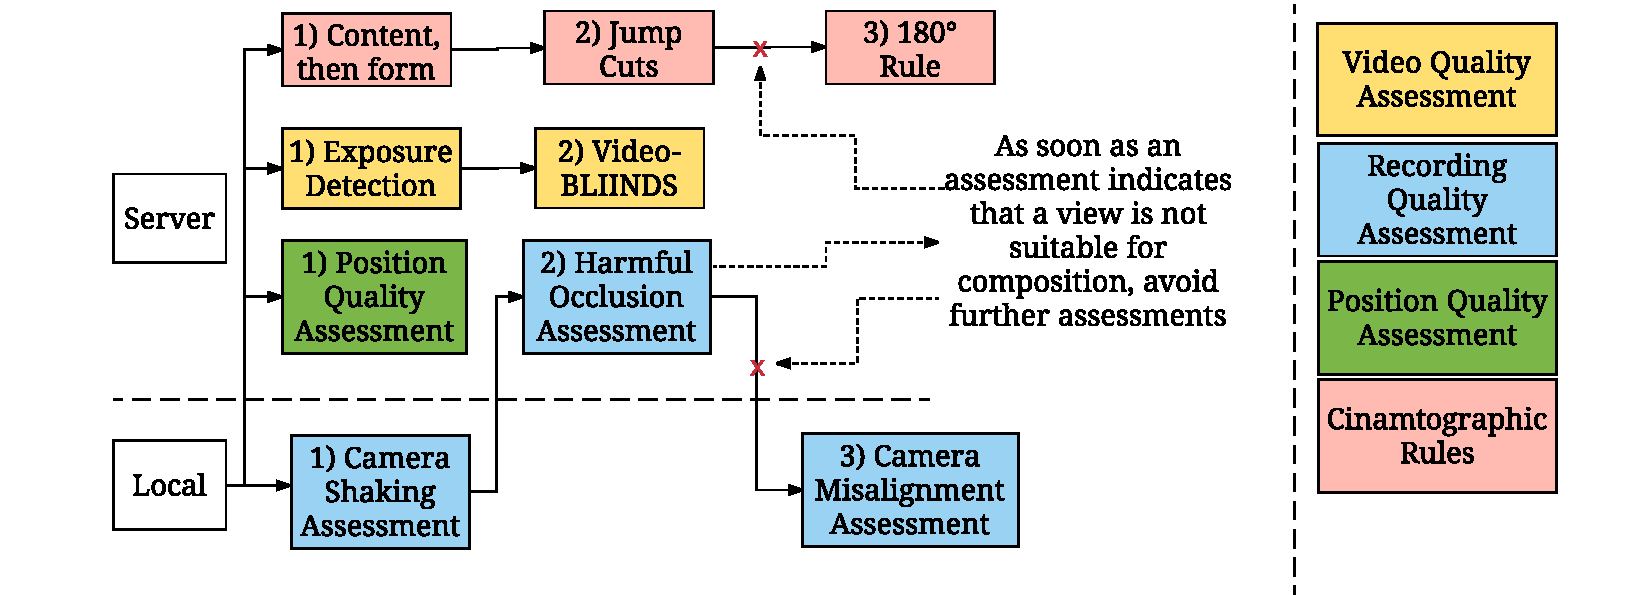
\includegraphics[width=\linewidth]{gfx/600_Composition/QualityAssessmentPipeline}
	\caption[Overview of quality assessment steps in the filter stage]{Filter Stage: Quality assessment pipeline for position quality, video quality and recording quality assessment as well as cinematographic rules.}
	\label{fig:617_qualityassessmentpipeline}
\end{figure}
\subsection{LiViU for Video Upload}
Before a quality assessment can be executed in the sequential pipelines shown in Figure~\ref{fig:617_qualityassessmentpipeline}, 
\ac{LiViU} is used for the upload of video streams.
The main task of \ac{LiViU} in the context of video composition is to upload a stream to the video composition component, which is run on a central server. 
During the process of uploading a video stream, the filter stage of the video composition application is triggered, determining the views that will not be selected for composition.
The filter stage of the video composition application leverages \ac{LiViU}'s capabilities to push or pull video streams. 
\subsection{Quality Assessment using the PaSC}
The \ac{PaSC} and related algorithms proposed in Chapter~\ref{chapter:550_scalable_quality_assessment} are used for quality assessment in the categories recording quality assessment and video quality assessment. % and audio quality assessment.
The reader should be aware, that the sequential pipeline of quality assessments is executed in a distributed manner which means that individual assessment steps are performed on different devices.

The sequential pipeline is constructed in a prioritized manner, with the most distracting degradations (i.e., in the recording quality assessment) analyzed first.
The recording quality assessment algorithms discussed here were introduced in Chapter~\ref{chapter:550_scalable_quality_assessment}.
The video quality assessment uses two complementary algorithms for under-/overexposition detection of video frames, as proposed by Saini et al.~\cite{Saini2012} and the \ac{V-BLIINDS} algorithm~\cite{Saad2012}.
\subsection{Recording Position Quality Assessment}
\label{sec:617_recordingQualityLocation}
Recordings of the same scene differ regarding the distance to a scene and the recording angle.
Chapter~\ref{chapter:400_RecordingQuality} proposed novel models that quantify the perceived quality in relation to its position.

Detection of a scene location is conducted using the novel \ac{AoI} algorithms as proposed in Section~\ref{sec:554_misalignments}.
It leverages the compass readings from the recording smartphones and camera lense information to determine the \ac{FoV} of all recording devices.
On the basis of the \ac{FoV} of many devices, the \ac{AoI} can be determined.
For determining the position of devices such as smartphones, a location provider is assumed, which offers reliable detection rates, such as \ac{GPS}. 
To compensate for varying reliabilities of the location providers, the quality models are mapped into a relative scene model (depicted in Figure~\ref{fig:617_ac_location}).
It classifies the distances of recorders in the audience in relation to each other into close to the scene (f), central (c) or in the back (b); and the angle into left (l), right (r) and central (c).
Zones are annotated with genre-specific quality values on the basis of the discussion in Chapter~\ref{chapter:400_RecordingQuality}.
This complete model gives no precise information on absolute positions and distances, but allows for a relative localization to cope with small imprecisions in smartphone sensors.

\begin{figure}
	\centering
	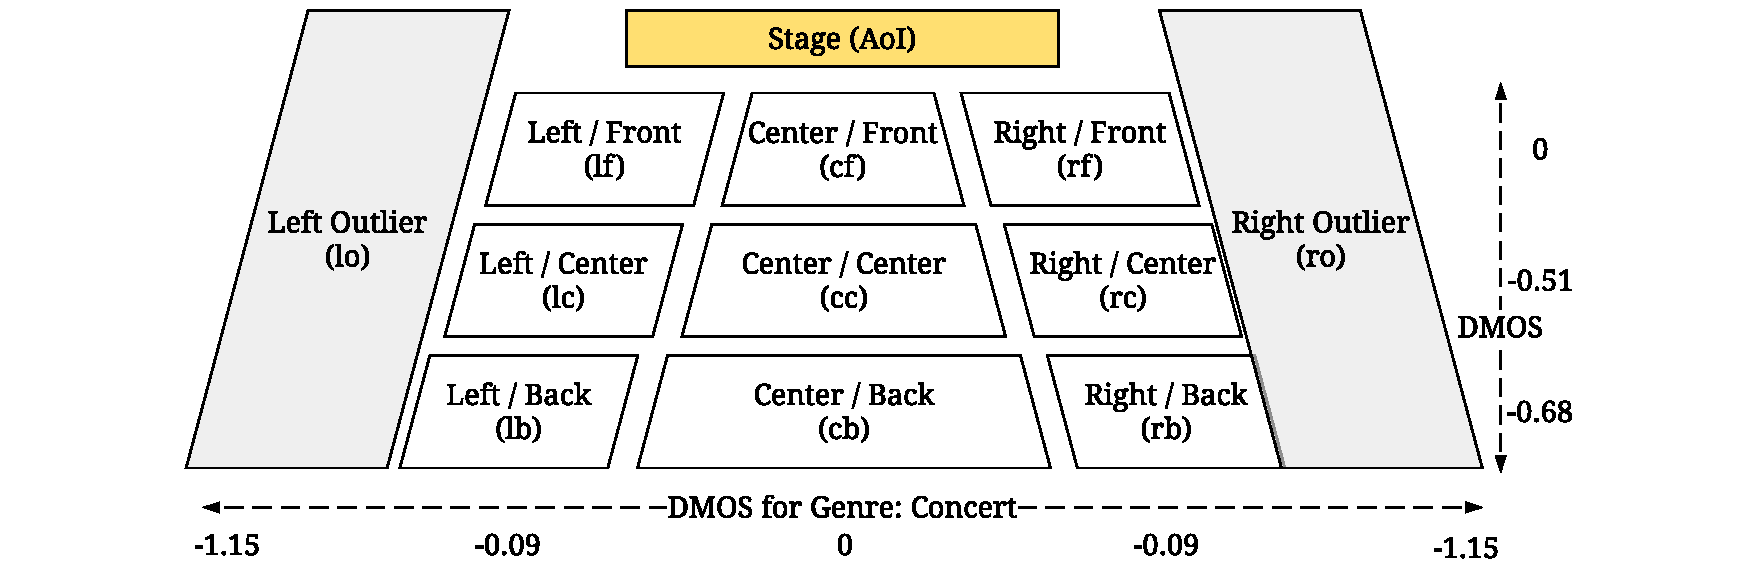
\includegraphics[width=\linewidth]{./gfx/600_Composition/OrientationLocation}%}
	\caption[Scene model used for the video composition]{Mapping of recording location based on the recording distance and angle from event to a relative scene model, including the impact of the recording position on the perceived quality [\ac{DMOS}].}
	\label{fig:617_ac_location}
\end{figure}
Indoor events require additional processing for retrieving the relative location of the recording devices.
Systems that achieve a suitable detection of relative positions rely on \acf{SfM} and have been evaluated in the context of video composition by Arev et al.~\cite{Arev2014}.
\subsection{Cinematographic Rules}
By the scene model discussed in the previous section, the cinematographic rules "content, then form," "$180\degree$ rule," and "jump cuts" are validated.
The camera misalignment algorithm as proposed in Section~\ref{sec:554_misalignments} is leveraged for scene localization.
It relies on a majority consensus decision, which excludes recordings which do not capture the \ac{AoI}.
The agreement on an \ac{AoI} allows to ensure that cinematographic rules are not broken for automatic video composition.

\emph{"Jump cut"} detection relies on the zones determined in the scene model.
As a result, when switching from one recorder to another, the new view shall not be captured within the same zone as the current recording.
Also, it is combined with the "$30\degree$ rule," which ensures that the relative angle between two recording positions should be at least $30\degree$.

Similarly, for detecting if the recorded views comply with the "$180\degree$ rule," the filter stage leverages the scene model and the orientation used by the built-in compass of the recording devices.
On the basis of this information, those views are detected which have been captured from an opposite direction.
These views are discarded from composition.